\chapter{Simulation results}
\label{chap:simulation}

In this chapter, I simulate the matching process of a labor market, using real
data on
workers' and firms' characteristics and assigned model parameters. I then apply
the two-sided logit model to show that the model is able to recover the
underlying parameters and to diagnose the properties of the MCMC sampling. I
compare the results of the two-sided logit model with the one-sided conditional
logit model, showing that the one-sided approach produces biased estimates of
workers' and firms' preference. This result demonstrates how the one-sided
approach, despite being the default method for analyzing two-sided markets, can
be misleading and unable to disentangle the effect of one side's preference from
the other side's.

\section{Labor market data}

To ensure that my simulation result generalizes to real situations, I use real
data on workers' and firms' characteristics from the US General Social Survey
(GSS), 1982-1990.\footnote{I thank Professor Michael Newton and Professor John
  Allen Logan for sharing the dataset.} On one side of the matching market is 2149 workers, a representative sample
of US male workers between 25 and 44 years old.
Table~\ref{tab:labor_occ5_summary_employee} shows the summary statistics for
workers. On average, a worker is 33 ($\pm$ 5.7)
years old and has 13 years ($\pm$ 3.1) of education. 11\% of workers in our sample are
non-white.

\begin{table}[!ht]
  \centering
  \caption{Summary statistics of workers' education, age, and race. The data
    come from the GSS, 1982-1990, for male workers in the US between 25 and 44
    years old.}
  \label{tab:labor_occ5_summary_employee}

% Table created by stargazer v.5.2 by Marek Hlavac, Harvard University. E-mail: hlavac at fas.harvard.edu
% Date and time: Mon, Apr 02, 2018 - 13:50:38
\begin{tabular}{@{\extracolsep{5pt}}lccccc} 
\\[-1.8ex]\hline 
\hline \\[-1.8ex] 
Statistic & \multicolumn{1}{c}{N} & \multicolumn{1}{c}{Mean} & \multicolumn{1}{c}{St. Dev.} & \multicolumn{1}{c}{Min} & \multicolumn{1}{c}{Max} \\ 
\hline \\[-1.8ex] 
Years of education & 2,149 & 13.103 & 3.111 & 2 & 20 \\ 
Age & 2,149 & 33.524 & 5.716 & 25 & 44 \\ 
Non-white & 2,149 & 0.113 & 0.316 & 0 & 1 \\ 
\hline \\[-1.8ex] 
\end{tabular} 

\end{table}

On the other side of the matching market are five firms, representing five job categories:
professional, managerial, sales / clerical / services, manufacturing blue
collar, and other blue collar. Table~\ref{tab:labor_occ5_summary_employer} shows
their characteristics. \textit{Prestige} is the Hodge-Seigel-Rossi score, used
in the GSS to measure the prestige of a job \citep{Hodge1964,
  NORC2014}. \textit{Autonomy} is calculated as the odds of having a supervisor, multiplied
by -1 so that a higher score is associated with a higher level of
autonomy.\footnote{In other words, $\text{autonomy} = -\frac{P(\text{having a
      supervisor})}{P(\text{not having a supervisor})}$} The prestige and the
autonomy scores of a firm in our dataset is the average scores reported by
workers who currently work in that job categories. Unemployment by itself does
not have a prestige and autonomy score. Following \citet{Logan1996}'s study on
the labor matching market, I calculate them as 50\%
of the prestige of the last job held and as the average autonomy scores of all
workers \citep{Logan1996}.\footnote{Our measurement of firms' prestige may be
  biased if workers that have a high regard for a certain type of job tend to
  work in that kind of job. Here we are making the assumption that workers are
  largely homogeneous so that workers in different jobs still have the same
  opinion regarding a job's prestige. While it is a strong assumption, it is not
an extra burden since we have already assumed that workers have the same set
of preferences in the modeling step. In addition, in other applications, such
as the FDI market where MNCs are matched with countries, we can obtain objective
data on countries' GDP, growth, and human capital, etc.}

\begin{table}[!ht]
  \centering
  \caption{Firms' characteristics}
  \label{tab:labor_occ5_summary_employer}

% Table created by stargazer v.5.2 by Marek Hlavac, Harvard University. E-mail: hlavac at fas.harvard.edu
% Date and time: Mon, Apr 02, 2018 - 13:50:38
\begin{tabular}{@{\extracolsep{5pt}} lccc} 
\\[-1.8ex]\hline 
\hline \\[-1.8ex] 
Firm category & Prestige & Pr(Supervisor) & Autonomy \\ 
\hline \\[-1.8ex] 
Unemployment & $18$ & $0.204$ & $$-$0.256$ \\ 
Professional & $59.670$ & $0.163$ & $$-$0.483$ \\ 
Managerial & $48.141$ & $0.442$ & $$-$3.237$ \\ 
Sales, Clerical, Services & $34.545$ & $0.100$ & $$-$0.112$ \\ 
Manufacturing Blue Collar & $34.330$ & $0.071$ & $$-$0.077$ \\ 
Other Blue Collar & $34.035$ & $0.175$ & $$-$0.214$ \\ 
\hline \\[-1.8ex] 
\end{tabular} 

\end{table}

\section{Simulated matching process}

I assign values to workers' and firms' preference parameters, choosing values to
achieve some level of realism and to have a sample of workers in each job.
Table~\ref{tab:sim_labor_nojobs_utility_functions} describes the utility
functions. I normalize firms' utility of not hiring to 0 so that firm $j$ will
extend and offer to worker $i$ if the utility of hiring is positive (i.e.
$U_{j}(i) > 0$. The magnitude of the intercept can thus be interpreted as how
selective a firm is in making an offer. For example, professional and managerial
firms are highly selective with intercepts of $-24$ and $-22$, while the other
firms are less so with intercepts of $-9, -8$ and $-6$. The coefficients
represent how much a firm values a worker's trait. For example, managerial and
professional firms have a similar preference for a worker's education, with
coefficients of 1 and 1.3. On the other hand, managerial firm values a worker's age twice
as much as professional firm does, with coefficients of 0.2 and 0.1.

While the two-sided logit model can be extended to accommodate different worker types as well, for
this simulation I assume that workers have homogeneous preference, sharing one
utility function.

Each utility function has a random component, represented by the
Gumbel-distributed error term $\epsilon$. While normally distributed error is
more common in simulations, justified by the claim that the error term is
the sum of many independent unobserved variables, here I use the Gumbel
distribution so that the coefficient estimates from the two-sided logit model can be
directly compared with the true preference parameter values.\footnote{If I use
  normally distributed error terms, the coefficient estimates have to be divided
by $\frac{\pi^2}{3}$ to be comparable with the true values.} Practically the
Gumbel distribution is very similar to the normal distribution, and I discussed
the implication of using the Gumbel distribution in further depth in Section~\ref{sec:model_firm_decision_making}.

\begin{table}[!ht]
\centering
\caption[Utility functions used in labor market simulations.]{Utility functions
  of firms and workers used in labor market simulation. $x_{i1}, x_{i2}, x_{i3}$ are worker \textit{i}'s education, age, and race (nonwhite is coded as 1). $w_{j1}, w_{j2}$ are firm \textit{j}'s prestige and autonomy, with $j \in \{1, \dots, 5\}$. The $\epsilon$'s are Gumbel-distributed error terms.}
\label{tab:sim_labor_nojobs_utility_functions}
\begin{tabular}{lll}
\\[-1.8ex]\hline
\textbf{Firms' utility functions}  &                                                                                     \\
Professional                         & $U_{j}(i) = -24 + 1.3 x_{i1} + 0.1 x_{i2} + 1 x_{i3} + \epsilon$         \\
Managerial                           & $U_{j}(i) = -22 + 1 x_{i1} + 0.2 x_{i2} + 1 x_{i3} + \epsilon$     \\
Sales, Clerical, Services            & $U_{j}(i) = -9 + 0.75 x_{i1} + -0.05 x_{i2} + 0 x_{i3} + \epsilon$ \\
Manufacturing blue collar            & $U_{j}(i) = -8 + 0.5 x_{i1} + 0.02 x_{i2} + 0 x_{i3} + \epsilon$   \\
Other blue collar                    & $U_{j}(i) = -6 + 0.5 x_{i1} - 0.01 x_{i2} + 1 x_{i3} + \epsilon$   \\
  \hline
\textbf{Workers' utility function} & $V_{i}(j) = 0.01 w_{j1} + 0.1 w_{j2} + \epsilon$                   \\
  \hline
\end{tabular}
\end{table}

With these utility functions, I simulate the matching process as follows:

\begin{itemize}
\item{First stage:} Each firm $j$ evaluates each worker $i$, calculating the utility of
  hiring. If the utility of hiring is positive, it will extend an offer.
  Unemployment is always an option for workers, and is thought of as a ``firm''
  that extends an offer to every worker. After
  this stage, we generate an opportunity set that is a $2149 \times 6$ matrix,
  in which cell $(i, j)$ is 1 if worker $i$ receives an offer from firm $j$ and
  0 if not. We typically do not observe this opportunity set matrix in real datasets.
\item{Second stage:} Worker $i$ evaluates each firm that extends him an offer in
  the first stage, calculating the utility of working for that firm. Worker $i$
  then chooses a firm (or unemployment) if it offers the highest utility. After this
  stage, we generate a choice vector that is a $2149 \times 1$ vector, in which
  cell $i$ equals $j$ if worker $i$ decides to work at firm $j$. This choice
  vector is what we observe in real datasets such as the GSS.
\end{itemize}

\section{Simulation results}

I estimate the two-sided logit model using the MCMC approach described in
Chapter~\ref{chap:model}. I use $N(0, \text{sd}=10)$ as a weak and proper prior for the preference
parameters. The results below are from a MCMC chain of 50,000
iterations with a thinning interval of 5, resulting in 10,000 saved iterations.
To propose new samples in the Metropolis-Hastings algorithm, I use normal
distributions with a scale hand-picked by examining the trace plots of discarded runs.

Figure~\ref{fig:sim_labor_nojobs_alpha} shows the trace plots of the MCMC
samples for workers' preference. We see that the MCMC chain mixes well and
quickly converge to the true value indicated by the red line. This result gives
us confidence that the MCMC algorithm is implemented correctly and can achieve
convergence within a reasonable time frame.

\begin{figure}[!ht]
  \centering
  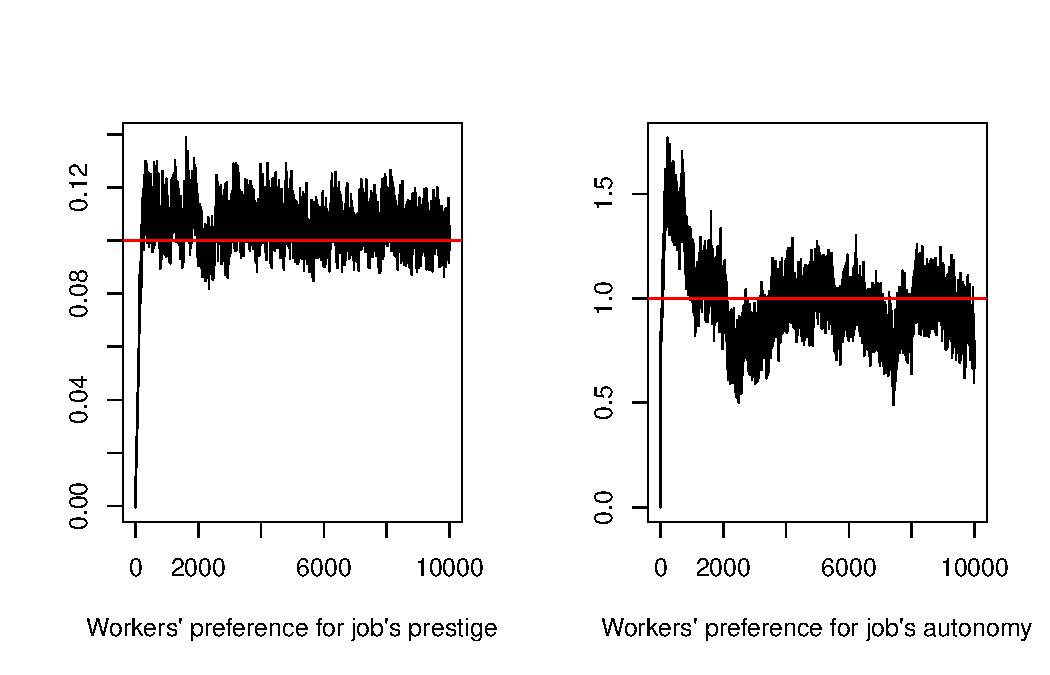
\includegraphics[width=\textwidth,keepaspectratio]{../figure/sim_labor_nojobs_alpha}
  \caption[Simulation result, estimate for workers' preference]{Two-sided logit estimates for workers' preference. The black line
    plots are the trace plots of the MCMC samplers, and the red line indicates the
    true parameter values. The trace plots show that the MCMC chain is able to
    converge to the true value after 10,000 iterations (2,000 saved iterations $\times 5$ thinning interval).}
  \label{fig:sim_labor_nojobs_alpha}
\end{figure}

Figure~\ref{fig:sim_labor_nojobs_beta_emp2} shows the trace plots of the MCMC
samples for professional firm's preference. We see that the MCMC chain is also
able to converge to the true parameter values, albeit slower and with more
autocorrelation between iterations.\footnote{To improve the mixing of the MCMC
  chain, I standardize workers' characteristics so that they have mean 0.
  Therefore, the intercept term has to be changed accordingly. The true
  intercept values displayed in the plots are the standardized intercepts, which
  is different from those reported in Table~\ref{tab:sim_labor_nojobs_utility_functions}.} There are several reasons for this poorer
mixing.

\begin{figure}[!ht]
  \centering
  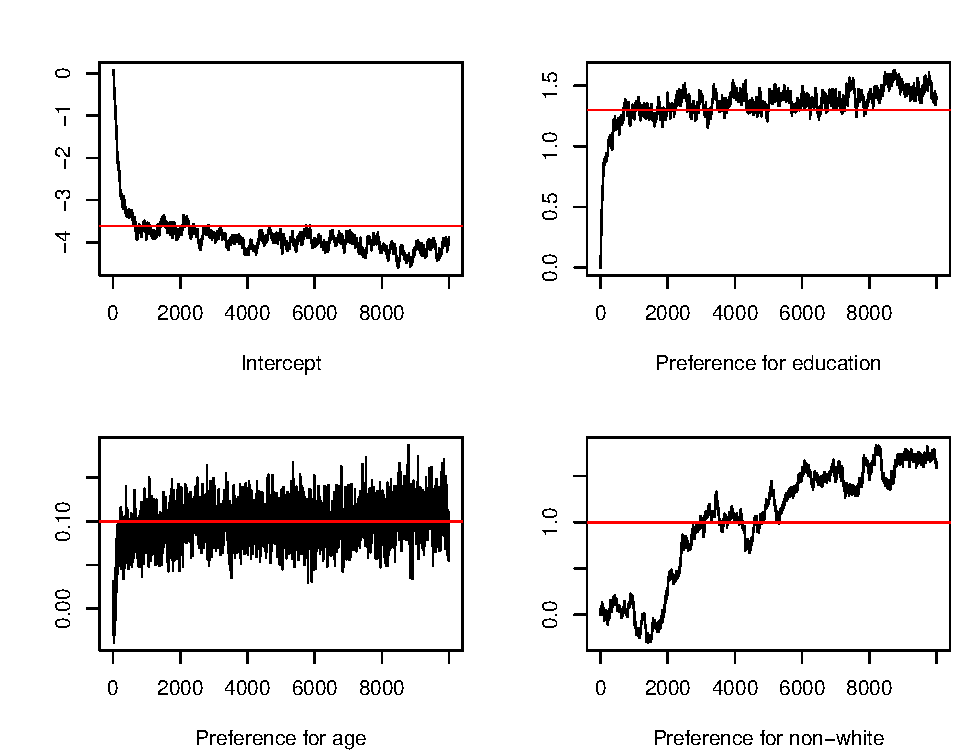
\includegraphics[width=\textwidth,keepaspectratio]{../figure/sim_labor_nojobs_beta_emp2}
  \caption[Simulation, estimates for professional firm's preference.]{Two-sided logit estimates for professional firm's preference. The
    MCMC chain is able to converge to the true parameter value, indicated by the
  red line, albeit with more autocorrelation than the MCMC chain for worker's
  preference in Figure~\ref{fig:sim_labor_nojobs_alpha}.}
  \label{fig:sim_labor_nojobs_beta_emp2}
\end{figure}

First, while we can use the entire sample to estimate the preference of
workers, only a subset of the sample works at a particular firm, resulting in a
smaller sample that we can use to estimate each firm's preference. This problem
is clearest in the trace plots for the managerial employer, which only has a
sample of 40 workers, or 1.9\% of the total sample \. To partially
combat this issue, I use a hierarchical model in which firms' preference
parameters are drawn from a common distribution. By doing so, I ``partially
pool'' the sample across firms, pulling the estimate for firms with small sample
sizes towards the common mean, and thus producing estimates that have more
predictive power \citep{Gelman2006}. On a related note, the MCMC chain of the
preference parameter for \textit{non-white} has a particularly poor mixing,
likely because \textit{non-white} is a binary variable, having less variation
and thus information that our model can use.

\begin{figure}[!ht]
  \centering
  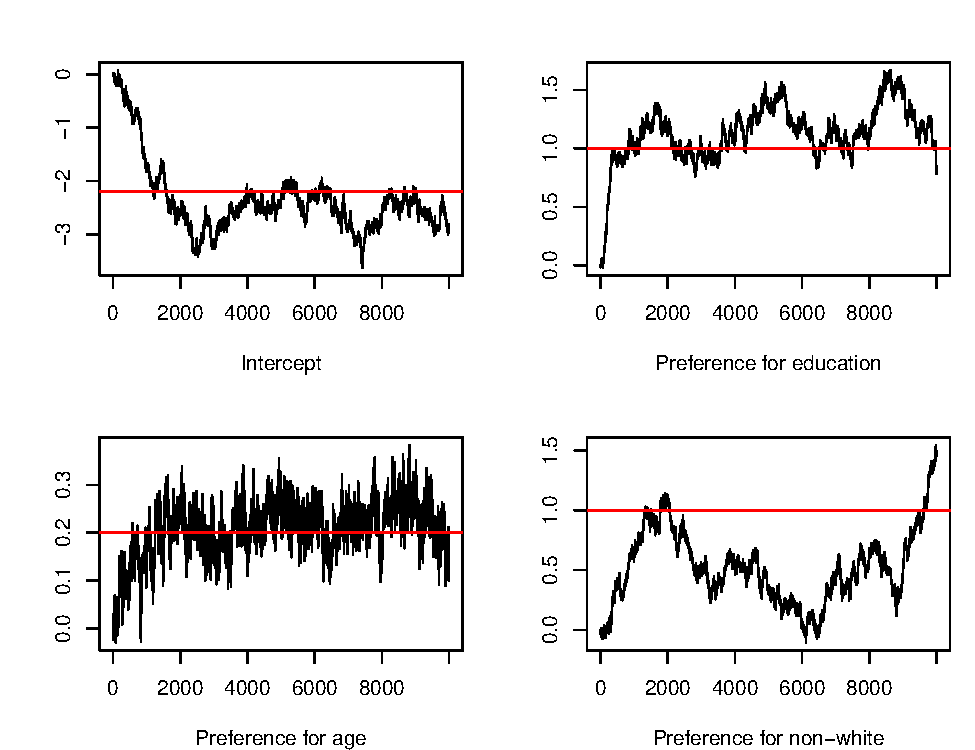
\includegraphics[width=\textwidth,keepaspectratio]{../figure/sim_labor_nojobs_beta_emp3}
  \caption[Simulation, poor mixing due to small sample size.]{Two-sided logit
    estimates for managerial firm's preference. Because the managerial firm only
  has a small sample size of 40 workers, or 1.9\% of the total sample, its
  preference is estimated more poorly than other's.}
  \label{fig:sim_labor_nojobs_beta_emp3}
\end{figure}

Second, while workers only have two preference parameters (for firm's prestige and autonomy), each firm has four
preference parameters (for worker's education, age, race, and an intercept
term), resulting in a total of 24 parameters. Updating the MCMC chain in such
high dimension is inherently difficult---to update one parameter we only need to
come up with one good proposal, but to update 24 parameters we need to come up
with good proposals for each of them.

Third, while firms' preference and the opportunity set are highly correlated,
our proposals for these parameters are independent, not take into their
correlation, and thus causing the MCMC to get stuck at local mode.
Section~\ref{sec:simulation_beta_opp_correlation} discusses this issue and
potential remedies in more details.

\section{Comparing two-sided logit model and one-sided models}

In this section, I demonstrate that, without taking into account the two-sided
nature of the matching market, one-sided models produce biased estimates of the
actors' preference. While it may be unsurprising that one-sided models fail when
the data generating process is so different from their assumptions, this is a
worthwhile exercise given that many empirical researches rely on these models.
For example, using discrete choice models (multinomial logit, conditional
logit), \citet{Cheng2006} models Japanese MNCs' location
choice across Chinese provinces and \citet{Aw2008} models Taiwanese firms' decision to
stay home or to open a factory in China and the US.\footnote{In the empirical literature,
  researchers often use the term ``multinomial logit'' and ``conditional logit''
interchangeably to refer to a discrete choice model of unordered choices.
In this discussion, I follow the terminology in \citet{McFadden1974}'s seminal paper on discrete
choice models, distinguishing ``multinomial logit'' as the model whose
independent variables are the choosers' characteristics, and ``conditional
logit'' as the model whose independent variables are the choices' characteristics.} Using count models (Poisson, negative
binomial), \citet{Wu1999} models MNCs' location choice in Guangzhou, China.
\citet{Arauzo-Carod2010} provides a literature review of how these methods are used in
studying the location choice of firms.

I estimate a conditional logit model in which workers choose the best firm to work
for as if all firms were available in their opportunity set. This assumption is
not satisfied by our two-sided data generating process. Figure~\ref{fig:sim_labor_nojobs_alpha_tsl_vs_cl} shows that the one-sided
conditional logit model is not robust when this assumption is violated,
producing biased estimates of workers' preference. Worse yet, its estimate has
little uncertainty and can cause researchers to be overly confident in the wrong
result.\footnote{This conditional logit model is equivalent to a Poisson model
  in which the dependent variable is the count of workers at each firm, as shown in
\citet{Guimaraes2003}. Both models, estimated with MLE, would produce exactly
the same estimates for the coefficients and their covariance matrix.
Therefore, the argument against one-sided logit applies fully to Poisson.}

\begin{figure}[!ht]
  \centering
  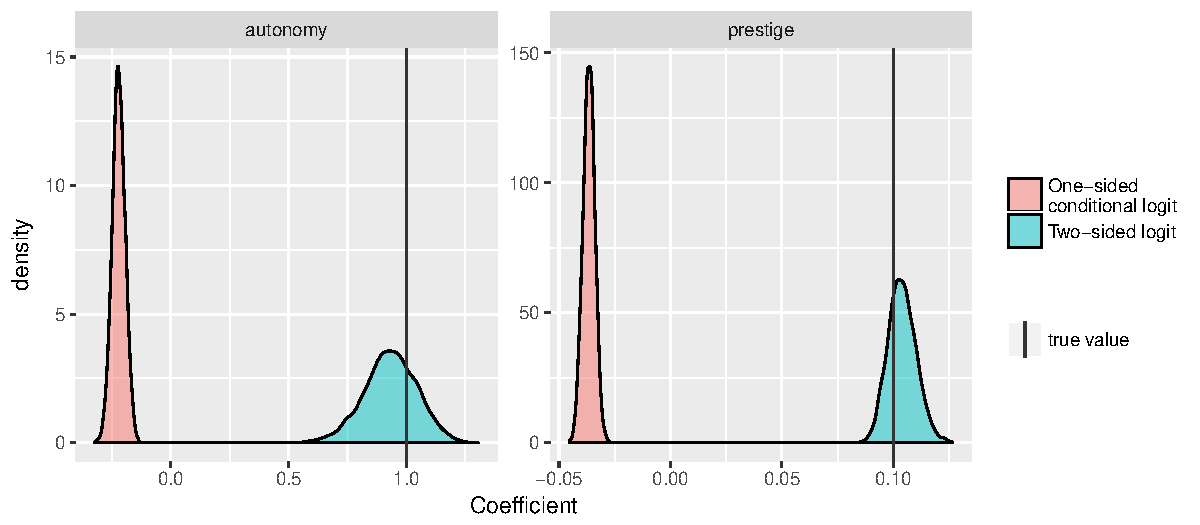
\includegraphics[width=\textwidth,keepaspectratio]{../figure/sim_labor_nojobs_alpha_tsl_vs_cl}
  \caption[Simulation, comparing the two-sided logit's and the
  one-sided conditional logit's estimate.]{Estimates of workers' preference,
    produced by two-sided logit and conditional logit. The density plots show
    that the two-sided logit's 95\% credible interval includes the true value,
    indicated by the black line, while the conditional logit's 95\% confidence
    interval is far from it.}
  \label{fig:sim_labor_nojobs_alpha_tsl_vs_cl}
\end{figure}

Examining the big difference between the two-sided and one-sided estimates for
\textit{prestige} demonstrates a situation in which the one-sided approach
confounds one side's preference with the other's. Figure~\ref{fig:sim_labor_nojobs_trueopp_obschoice} (left) shows the binary heat map
for the true opportunity set---a dark blue cell indicates that an offer is made by firm in
column $j$ to worker in row $i$. The columns for professional and
managerial firms are quite similar, reflecting the fact that they make offers to
the same kind of workers. In contrast, in the observed choice
(Figure~\ref{fig:sim_labor_nojobs_trueopp_obschoice}, right), the columns for
professional and managerial firms are very different,
reflecting the fact that the professional firm is slightly more
desirable, causing workers that receive offers from both firms to
overwhelmingly choose to work for the professional firm 
over the managerial firm. Therefore, there are very few workers at the
managerial firm. To the one-sided conditional
logit model, it looks
as if the managerial firm---a highly prestigious job---were less desirable than
even the services and blue collar firms. Therefore, it severely underestimate
workers' preference for \textit{prestige} to such an extent that
\textit{prestige} is considered a negative trait. This example shows how
misleading it can be to estimate workers' preference by assuming that all the
choices are available. Indeed, the managerial firm is rarely chosen not because
it is undesirable, but because it has to compete with the professional firm for
the same pool of highly educated and experienced workers.

\begin{figure}[!ht]
  \centering
  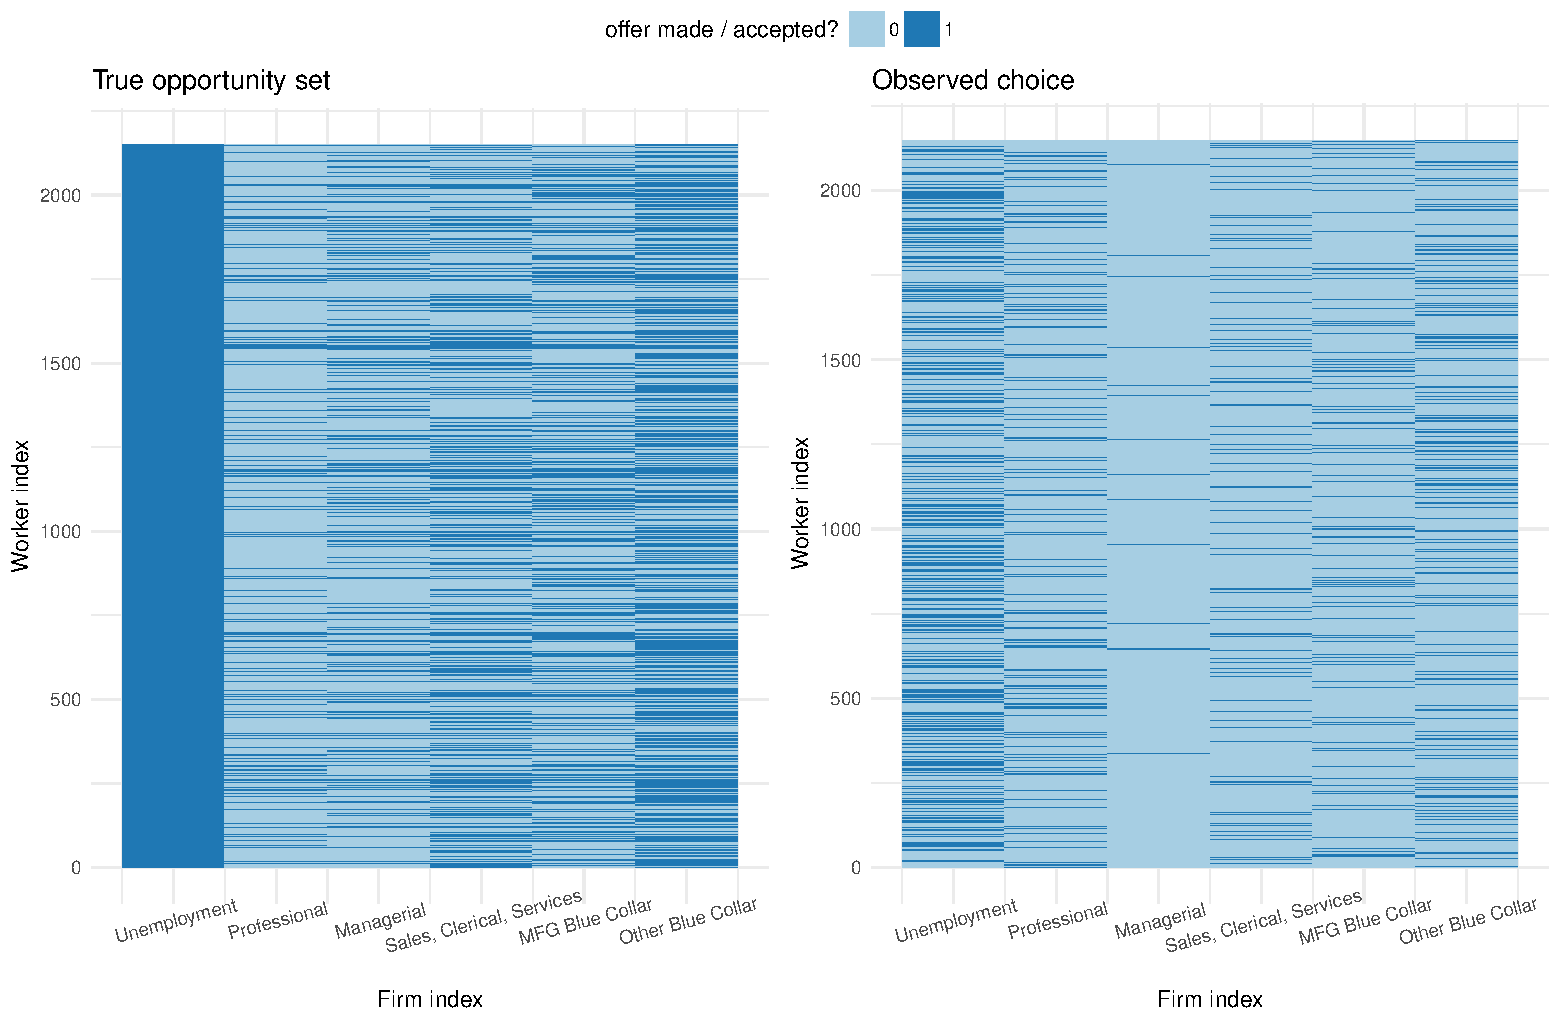
\includegraphics[width=\textwidth,keepaspectratio]{../figure/sim_labor_nojobs_trueopp_obschoice}
  \caption{Binary heat map for the true opportunity set (left) and observed
    choice (right). A dark blue cell indicates that an offer was made (or accepted)
    between the firm in the corresponding column and the worker in the corresponding
    row.}
  \label{fig:sim_labor_nojobs_trueopp_obschoice}
\end{figure}

\section{Issues with MCMC convergence}
\label{sec:simulation_beta_opp_correlation}

The MCMC chain for firms' preference parameters $\beta$ is poorly mixed because
it is highly correlated with the opportunity set. Intuitively, at any point
during the MCMC, we cannot propose a new opportunity set that is very different
from the current one because it would be too unlikely given the current value of
$\beta$. Likewise, we cannot propose too different a value for $\beta$ because
it would be rejected given the current opportunity set.

This problem is especially severe for firms with only a few workers. If we
propose a new opportunity set in which those firms now extends the offer to a
new worker, then this new worker will heavily affect the estimate for $\beta$
especially if it is different from the current workers. In contrast, for firms
with a large sample size, there is already a lot of information to precisely estimate
their preference. Making one new offer in these cases will not substantially change the
estimate.

Currently, I make random-walk proposals for $\beta$ and the opportunity set,
which insufficiently takes into account this correlation, causing poor mixing. A
potential solution to this problem is to make a correlated proposal for $\beta$
and for the opportunity set: if we propose a new $\beta$ that
puts a high emphasis on workers' education, then we should also perturb the
opportunity set to make more offers to highly-educated worker. While
conceptually simple, this approach is not straightforward to implement, and is
left for future research.\footnote{Alternatively, we may reparameterize the
  model entirely and eliminate the opportunity set, whose binary nature makes it
impossible to use more modern MCMC approach such as Hamiltonian Monte Carlo. A
potential alternative parameterization is \citet{Logan2008}'s, which samples
directly from the utility space.}

%%% Local Variables:
%%% mode: latex
%%% TeX-master: "../AnhLe_dissertation.tex"
%%% End: